% !TeX root = ../main.tex

\chapter{Experimental Results and Analysis}\label{chapter:Experimental Results and Analysis}

This chapter presents the results by experimental factor. It first validates
the measurement procedure and then isolates the effects of message size, MPI
implementation, transport, progress mechanism, CPU-resource
configuration, and compute-window duration. Unless stated otherwise, each
comparison changes only the factor named in the corresponding section.

\section{Measurement Validation}

\label{sec:measurement-validation}

Each reported result is based on ten independent experimental runs.
Repeated measurements capture run-to-run variability, but do not eliminate
random timing fluctuations. Variations in network conditions, operating-system
scheduling, and other runtime effects may produce occasional peaks in the
measured communication times and the resulting overlap values. The measurements
do not isolate the contribution of each of these possible sources.

All measured values, including such peaks, are retained in the reported
statistics; observations are not discarded solely because they deviate markedly
from the other runs. The mean and the run-to-run range therefore preserve the
random variability observed across the ten runs. The subsequent analysis
considers this variability when interpreting differences between configurations
and trends across message sizes.

Table~\ref{tab:intelmpi-tcp-smallmsg-variability} illustrates this variability
for Intel MPI TCP at a peer payload of 1.56~KiB. Although each case contains
ten independent runs, substantial differences remain between individual
measurements.

\begin{table}[p]
    \centering
    \scriptsize
    \caption[Ten-run variability for Intel MPI TCP.]{Individual overlap
    results for Intel MPI TCP at a peer payload of 1.56~KiB.
    All ten runs use the same Mock-corrected communication cost of
    $30.282\,\mu\mathrm{s}$ as the normalization reference. The final rows
    report the minimum, mean, and maximum across the ten runs.}
    \label{tab:intelmpi-tcp-smallmsg-variability}
    \begin{tabular}{crr}
        \toprule
        Run & Case 01 (\%) & Case 03 (\%) \\
        \midrule
        run\_01 & 21.12  & 113.27 \\
        run\_02 & 39.16  & 39.87  \\
        run\_03 & 204.34 & 75.97  \\
        run\_04 & 61.69  & 67.58  \\
        run\_05 & 28.57  & 67.37  \\
        run\_06 & 45.53  & 133.35 \\
        run\_07 & 37.72  & 57.11  \\
        run\_08 & 39.91  & 57.57  \\
        run\_09 & 40.63  & 67.85  \\
        run\_10 & 53.59  & 36.54  \\
        \midrule
        Min  & 21.12  & 36.54  \\
        Mean & 57.23  & 71.65  \\
        Max  & 204.34 & 133.35 \\
        \bottomrule
    \end{tabular}
\end{table}

Case~01 ranges from 21.12\% to 204.34\%, with a mean of 57.23\%.
Run~03 produces a pronounced peak of 204.34\%, while the other nine
measurements lie between 21.12\% and 61.69\%. Case~03 also exhibits
substantial variation, ranging from 36.54\% to 133.35\%, with a mean
of 71.65\%; runs~01 and~06 both exceed 100\%. These results demonstrate
that ten independent runs do not eliminate large timing fluctuations
under the measured runtime conditions. Values above 100\% under this
normalization by the measured computation time do not imply physical overlap beyond the
compute window. All ten observations, including the peaks, are retained
in the statistics so that the reported results reflect this random
variability rather than suppressing it through outlier removal.

\section{Message Size and MPI Implementation}

\subsection{Mock-Corrected Communication Cost}

\autoref{tab:cost-2n2r-cm4-inter} reports the Mock-corrected communication
cost $\widehat{T}_{\mathrm{comm}}$, defined in
\autoref{sec:timing-metrics}, for the 19 payloads of the two-node,
two-rank \texttt{cm4\_inter} reference configuration. The results correspond
to Case~03 with asynchronous progress enabled, 23 application threads,
\texttt{wait\_all} completion, and the fully sequential
\texttt{seq/seq-seq} execution policy. Payload denotes the complete
aggregated message sent to the inter-node partner.

\begin{table}[!htbp]
    \centering
    \scriptsize
    \caption[Two-rank Mock-corrected communication cost.]{Mock-corrected
        communication cost for Case~03 with the \texttt{seq/seq-seq}
        policy in the \texttt{cm4\_inter} two-node, two-rank configuration.
        Values are in $\mu$s.}
    \label{tab:cost-2n2r-cm4-inter}
    \begin{tabular}{lrrrr}
        \toprule
        Peer payload & Intel verbs & Intel TCP & MPICH TCP & Open MPI TCP \\
        \midrule
        1.56 KiB   & 10.322   & 30.282   & 26.824   & 124.698  \\
        3.13 KiB   & 12.789   & 32.338   & 32.167   & 185.412  \\
        4.69 KiB   & 18.389   & 31.142   & 30.507   & 214.819  \\
        6.25 KiB   & 24.944   & 41.584   & 28.594   & 210.408  \\
        9.38 KiB   & 27.701   & 46.703   & 36.017   & 274.870  \\
        12.50 KiB  & 33.171   & 50.929   & 37.435   & 280.118  \\
        15.63 KiB  & 37.382   & 51.662   & 37.095   & 311.566  \\
        18.06 KiB  & 37.322   & 62.542   & 50.211   & 345.424  \\
        18.75 KiB  & 42.687   & 62.252   & 30.838   & 317.220  \\
        36.13 KiB  & 35.889   & 58.718   & 44.679   & 493.553  \\
        72.25 KiB  & 73.893   & 79.006   & 76.149   & 248.083  \\
        144.50 KiB & 100.000  & 64.543   & 177.998  & 208.448  \\
        289.00 KiB & 170.000  & 198.836  & 178.221  & 259.094  \\
        578.00 KiB & 230.676  & 373.755  & 269.086  & 200.423  \\
        1.13 MiB   & 501.483  & 838.070  & 405.400 & 267.775  \\
        2.26 MiB   & 746.096  & 1383.583 & 993.808  & 851.659  \\
        3.39 MiB   & 963.993  & 2509.543 & 1493.140 & 1143.607 \\
        4.52 MiB   & 1167.395 & 3420.671 & 2136.178 & 2061.891 \\
        5.93 MiB   & 2076.622 & 4090.282 & 3456.913 & 2980.504 \\
        \bottomrule
    \end{tabular}
\end{table}


Across the complete sweep, the exposed communication cost generally increases
with peer payload, but the magnitude and rate of increase differ substantially
between the MPI implementations and transport configurations. Intel MPI verbs
has the lowest cost over most of the small-message region, while Open MPI TCP
shows markedly higher communication cost at the smallest payloads. As the payload
increases, the differences between the TCP-based configurations become more
pronounced, with Intel MPI TCP showing the highest communication cost at the
upper end of the sweep.
The measured Mock-corrected communication cost does not increase linearly with
message size and can even decrease over some payload intervals, as observed for
Open MPI TCP.

These differences in communication baseline are important for the subsequent
overlap comparison because, even at the same peer payload, the communication
interval available to be hidden by computation differs between MPI
implementations. The implementation- and payload-specific compute targets
defined in \autoref{sec:timing-metrics} are therefore retained in the subsequent
overlap analysis rather than applying a common compute duration across the
complete message-size sweep.

The values in \autoref{tab:cost-2n2r-cm4-inter} are used primarily to
characterize the communication-cost scale and to support compute-window
calibration, rather than as high-precision estimates of the population mean.

\subsection{Overlap across Message Sizes}


\subsubsection{Open MPI}


\begin{figure}[p]
    \centering
    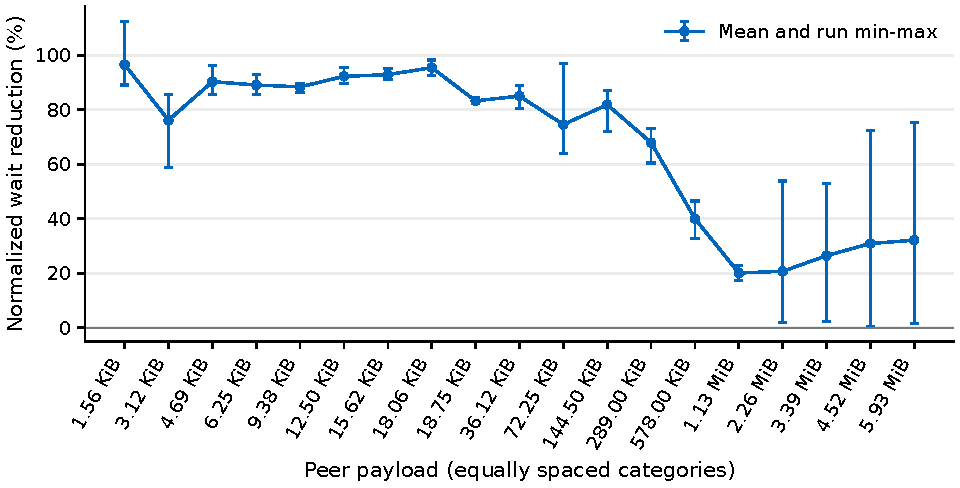
\includegraphics[width=0.9\textwidth]
    {figures/msgsize-vs-overlap/openmpi-case06-overlap-vs-message-size.pdf}
    \caption[Open MPI overlap across message sizes.]{Overlap across the
        19 peer payloads for Open MPI in the two-node, two-rank
        \texttt{cm4\_inter} configuration for Case~03. Open MPI uses the
        OB1 PML with the TCP BTL for inter-node communication, with
        asynchronous TCP progress enabled, 23 application threads, one CPU
        reserved for the progress thread, \texttt{wait\_all} completion,
        and the \texttt{seq/seq-seq} execution policy.}
    \label{fig:openmpi-case06-overlap-msgsize}
\end{figure}

Beyond 144.50~KiB, the overlap decreases progressively across several
consecutive payloads. The mean falls from approximately 82\% at
144.50~KiB to about 68\% at 289~KiB, 40\% at 578~KiB, and approximately
20\% at 1.13~MiB. Because this reduction extends across multiple
neighboring message sizes, it represents a systematic change in the
observed message-size behavior rather than an isolated data point.

For payloads above 1.13~MiB, the mean overlap remains at a substantially
lower level and shows only a limited recovery at larger message sizes.
At the same time, the run-to-run ranges are generally larger than in the
small-message region, indicating reduced stability of the overlap behavior
for large payloads.

The Open MPI TCP parameters provide additional context for this behavior.
The parameters were queried using \texttt{ompi\_info} in the same Open MPI
environment used for the experiments.\footnote{\texttt{ompi\_info --param
btl tcp --level 9}} The TCP BTL reports an eager limit of 64~KiB and a
maximum send size of 128~KiB. The first sampled payload above the eager
limit is 72.25~KiB, where a local reduction in overlap is visible.
However, the more pronounced and sustained decrease begins only at larger
payloads, beyond approximately 144.50~KiB.

This indicates that the eager-to-rendezvous transition alone is not
sufficient to explain the complete large-message trend. Although the onset
of the large-message regime is consistent with the first local change in
overlap, the continued degradation at larger payloads suggests that
additional large-message effects, such as sustained progress requirements
and increased data movement, may also contribute. The present measurements
do not isolate these mechanisms individually, so no single protocol
threshold is assigned as the definitive cause of the observed decrease.

\subsubsection{MPICH TCP}
\begin{figure}[htbp]
    \centering
    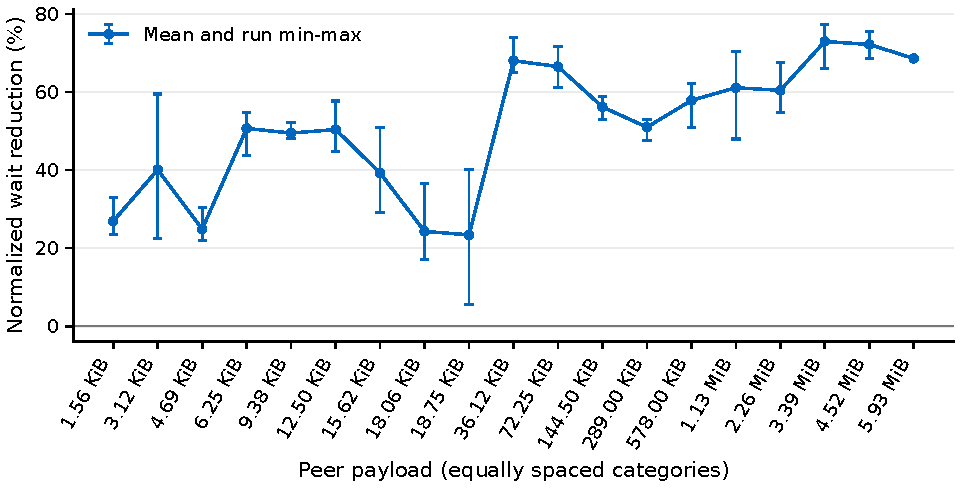
\includegraphics[width=0.9\textwidth]
    {figures/msgsize-vs-overlap/mpich-case06-overlap-vs-message-size.pdf}
    \caption[MPICH overlap across message sizes.]{Overlap across the
        19 peer payloads for MPICH TCP in the two-node, two-rank
        \texttt{cm4\_inter} configuration for Case~03, using
        \texttt{wait\_all} completion and the \texttt{seq/seq-seq}
        execution policy.}
    \label{fig:mpich-case06-overlap-msgsize}
\end{figure}

For MPICH TCP, the most notable message-size dependence appears in the
small-message region, where two pronounced local turning points are visible.
The overlap varies considerably across the smallest payloads rather than
following a monotonic trend.

Beyond the small-message region, MPICH achieves both higher and more stable
overlap. From approximately 36.12~KiB onward, the mean overlap generally
remains at a moderate to high level, and the large-message region shows
substantially less variation in the overall trend. In the MiB range, the mean
overlap is mostly maintained around 60\%--70\%, indicating that MPICH
preserves comparatively strong overlap even as the payload increases.

The MPICH results therefore differ from the Open MPI behavior observed above:
the main irregularities are concentrated at small payloads, whereas larger
messages exhibit a more stable and consistently higher degree of
communication--computation overlap.




\subsubsection{Intel MPI: verbs and TCP}

Figures~\ref{fig:intelmpi-verbs-case06-overlap-msgsize} and
\ref{fig:intelmpi-tcp-case06-overlap-msgsize} show the message-size
dependence of measured overlap for Intel MPI verbs and TCP with
asynchronous progress enabled (Case~03). Both configurations exhibit
irregular overlap at small payloads and generally higher overlap at
larger payloads, although their local variations differ.

For Intel MPI verbs, the mean overlap decreases from approximately 72\%
at 3.12~KiB to 57\% at 4.69~KiB and 46\% at 6.25~KiB, before recovering
at the following payloads. A further region of lower overlap extends
from 18.06~KiB to 72.25~KiB. The mean is approximately 59\% at
36.12~KiB and 41\% at 72.25~KiB, followed by a pronounced increase to
approximately 95\% at 144.50~KiB.

For Intel MPI TCP, local reductions are visible at 4.69~KiB and around
18.06--18.75~KiB. The mean overlap increases from approximately 59\% at
18.75~KiB to 89\% at 36.12~KiB, remains around 85\% at 72.25~KiB,
and reaches approximately 98\% at 144.50~KiB. Thus, the recovery occurs
at a smaller payload than for verbs.

From 144.50~KiB onward, both transports maintain comparatively high
measured overlap across the remaining sweep. Intel MPI verbs generally
remains near 100\%, while TCP mostly lies between approximately 83\%
and 103\%. Neither transport shows a sustained decline toward zero in
the large-payload region under the tested progress-enabled configuration.

\begin{figure}[htbp]
    \centering
    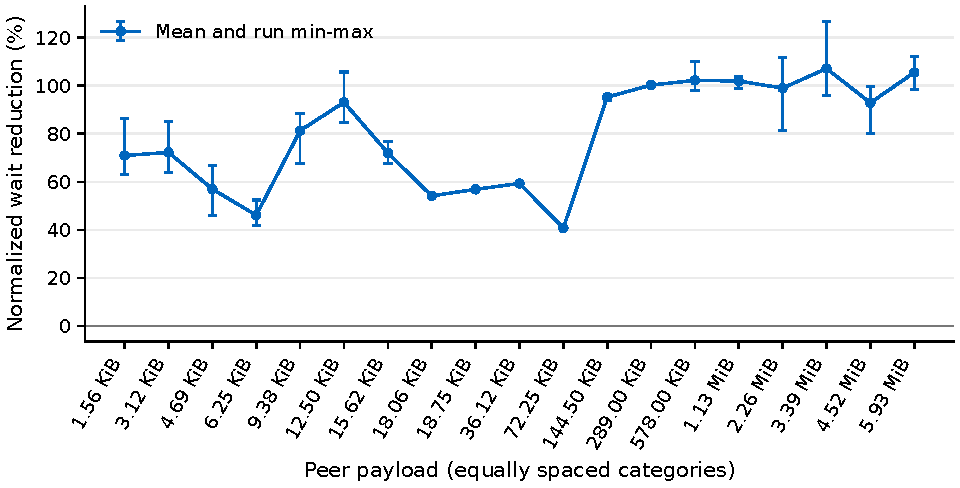
\includegraphics[width=0.9\textwidth]
    {figures/msgsize-vs-overlap/intelmpi-case06-overlap-vs-message-size.pdf}
    \caption[Intel MPI verbs overlap across message sizes.]{Overlap across the
        19 peer payloads for Intel MPI using the verbs transport in the
        two-node, two-rank \texttt{cm4\_inter} configuration for Case~03.}
    \label{fig:intelmpi-verbs-case06-overlap-msgsize}
\end{figure}

\begin{figure}[htbp]
    \centering
    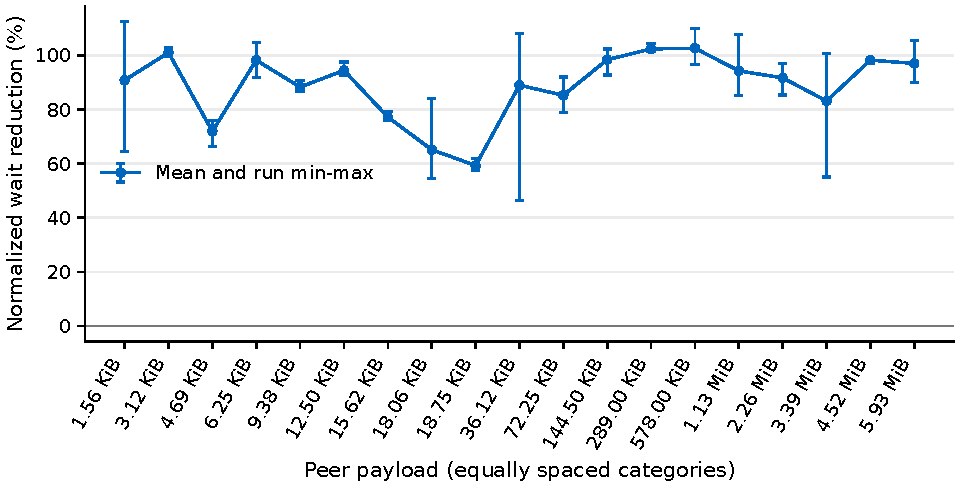
\includegraphics[width=0.9\textwidth]
    {figures/msgsize-vs-overlap/intelmpi_tcp-case06-overlap-vs-message-size.pdf}
    \caption[Intel MPI TCP overlap across message sizes.]{Overlap across the
        19 peer payloads for Intel MPI using TCP transport in the
        two-node, two-rank \texttt{cm4\_inter} configuration for Case~03.}
    \label{fig:intelmpi-tcp-case06-overlap-msgsize}
\end{figure}






\subsection{Cross-Implementation Comparison}
The message-size sweeps reveal two qualitatively different overlap patterns
across the evaluated MPI implementations. Intel MPI and MPICH both exhibit
pronounced irregularities in the small-message region, while medium and
large payloads generally achieve higher and more stable overlap. For Intel
MPI, this overall pattern is observed with both verbs and TCP transport,
indicating that the broad message-size dependence is not specific to a
single transport path.

Open MPI shows a different large-message behavior. Its overlap remains high
for small and medium payloads but decreases progressively once the payload
enters the larger-message range. Consequently, the relative behavior of the
implementations changes with message size: Open MPI performs strongly in the
small-message region, whereas Intel MPI and MPICH maintain substantially
higher overlap for large payloads.







\subsection{Asynchronous Progress}

\subsubsection{Open MPI}

\begin{figure}[htbp]
    \centering
    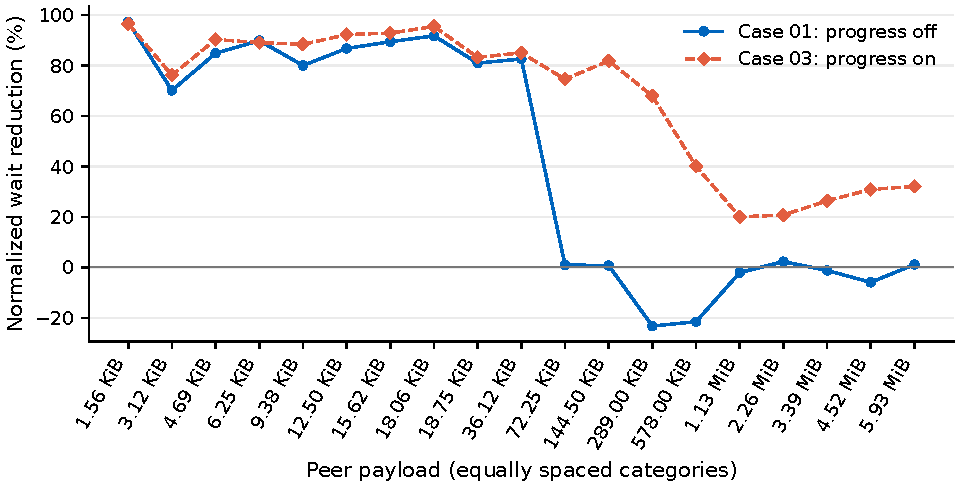
\includegraphics[width=\textwidth]{figures/on_off/inter-openmpi-case01-06-overlap-vs-message-size.pdf}
    \caption[Open MPI TCP asynchronous progress off versus on.]{Open MPI TCP: measured overlap across 19 peer payloads with
        asynchronous progress disabled (Case~01, solid line with circles,
        24 application threads) and enabled (Case~03, dashed line with diamonds,
        23 application threads and one CPU reserved for progress).
        Both cases use \texttt{wait\_all} and \texttt{seq/seq-seq} in the
        two-node, two-rank \texttt{cm4\_inter} configuration.}
    \label{fig:openmpi-progress-on-off}
\end{figure}


For Open MPI, asynchronous progress is not controlled by a single global
on/off switch. In the present experiments, Case~03 represents the
progress-thread configuration by enabling a dedicated TCP BTL progress
thread and reserving one CPU for it.\footnote{The Open MPI configuration
used \texttt{OMPI\_MCA\_btl\_tcp\_progress\_thread=1},
\texttt{OMPI\_MCA\_mpi\_yield\_when\_idle=0},
\texttt{OMPI\_MCA\_opal\_progress\_sched\_yield=0}, and
\texttt{OMPI\_MCA\_mpi\_add\_procs\_cutoff=0}.}

As shown in Figure~\ref{fig:openmpi-progress-on-off}, Case~01 and Case~03 exhibit
similar behavior in the small-message region. Up to approximately
36.12~KiB, both configurations generally maintain high overlap, with most
values between about 70\% and 95\%. This indicates that the TCP BTL
progress-thread configuration has a limited effect on Open MPI overlap
for smaller message payloads.

The first clear divergence occurs at 72.25~KiB. In Case~01, without a
dedicated TCP BTL progress thread, the mean overlap drops sharply from
approximately 83\% at 36.12~KiB to nearly zero at 72.25~KiB and remains
close to zero for most subsequent larger payloads. In contrast, Case~03
retains substantial overlap over the same message-size range. Although
the Case~03 overlap decreases as the payload increases, it remains
consistently higher than that of Case~01 throughout the medium- and
large-message region.

These results indicate that the Open MPI TCP BTL progress-thread
configuration has a limited effect in the small-message region, but
substantially improves communication--computation overlap for medium
and large message payloads.

\subsubsection{MPICH}

For MPICH, asynchronous progress is controlled through
\texttt{MPIR\_CVAR\_ASYNC\_PROGRESS}. Case~01 disables asynchronous
communication progress, whereas Case~03 enables the MPICH asynchronous progress
thread.\footnote{The MPICH configurations use
\texttt{MPIR\_CVAR\_ASYNC\_PROGRESS=0} for Case~01 and
\texttt{MPIR\_CVAR\_ASYNC\_PROGRESS=1} for Case~03. In the tested MPICH
build, enabling this variable creates one progress thread per MPI rank.}

\begin{figure}[htbp]
    \centering
    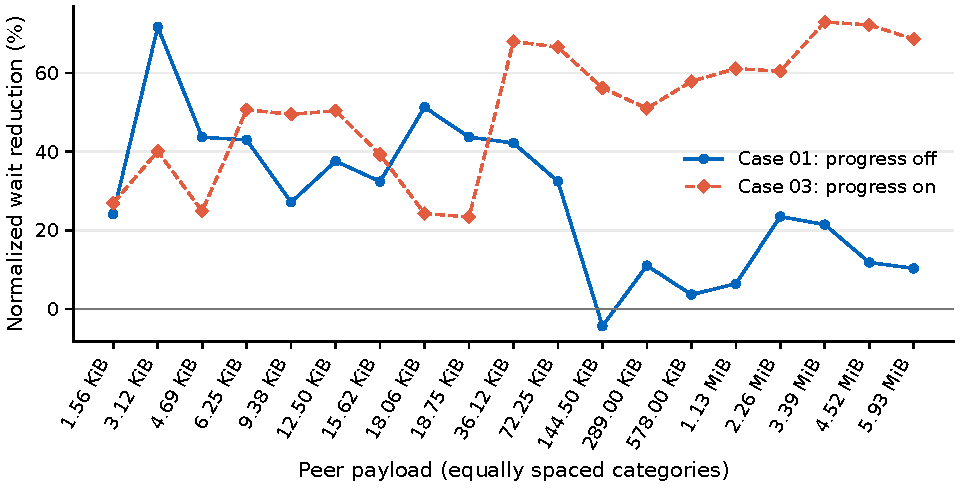
\includegraphics[width=\textwidth]{figures/on_off/inter-mpich-case01-06-overlap-vs-message-size.pdf}
    \caption[MPICH TCP asynchronous progress off versus on.]{MPICH TCP: measured overlap across 19 peer payloads with
        asynchronous progress disabled (Case~01, solid line with circles,
        24 application threads) and enabled (Case~03, dashed line with diamonds,
        23 application threads and one CPU reserved for progress).
        Both cases use \texttt{wait\_all} and \texttt{seq/seq-seq} in the
        two-node, two-rank \texttt{cm4\_inter} configuration.}
    \label{fig:mpich-progress-on-off}
\end{figure}

As shown in Figure~\ref{fig:mpich-progress-on-off}, both MPICH configurations
exhibit relatively irregular overlap behavior in the small-payload region.
Below 36.12~KiB, the effect of asynchronous progress is not consistent:
overlap varies substantially with peer payload size, and neither
configuration consistently outperforms the other across the entire
small-payload range.

A clearer difference between the two configurations emerges at 36.12~KiB
and persists across larger payloads. At 36.12~KiB, the mean overlap is
approximately 68\% for Case~03, compared with approximately 42\% for
Case~01. For subsequent larger payloads, Case~01 generally exhibits lower
overlap. Its mean overlap becomes slightly negative at 144.50~KiB and
remains mostly below approximately 25\% in the larger-payload region.

In contrast, Case~03 maintains substantially higher overlap over the same
range. From 36.12~KiB onward, its mean overlap mostly remains between
approximately 50\% and 70\%, exceeding 70\% at several of the largest
payload points.

These results indicate that enabling MPICH asynchronous progress does not
provide a consistent improvement for small payloads, but substantially
improves communication--computation overlap for medium and large payloads.


\subsubsection{Intel MPI}

For Intel MPI, asynchronous progress is controlled through
\texttt{I\_MPI\_ASYNC\_PROGRESS}. Case~01 disables asynchronous progress,
whereas Case~03 enables it and reserves one CPU for the progress
thread.\footnote{The Intel MPI configuration uses
\texttt{I\_MPI\_ASYNC\_PROGRESS=0} for Case~01 and
\texttt{I\_MPI\_ASYNC\_PROGRESS=1} for Case~03. For Case~03,
\texttt{I\_MPI\_ASYNC\_PROGRESS\_THREADS=1} is used, with one CPU reserved
for the progress thread.}

\begin{figure}[htbp]
    \centering
    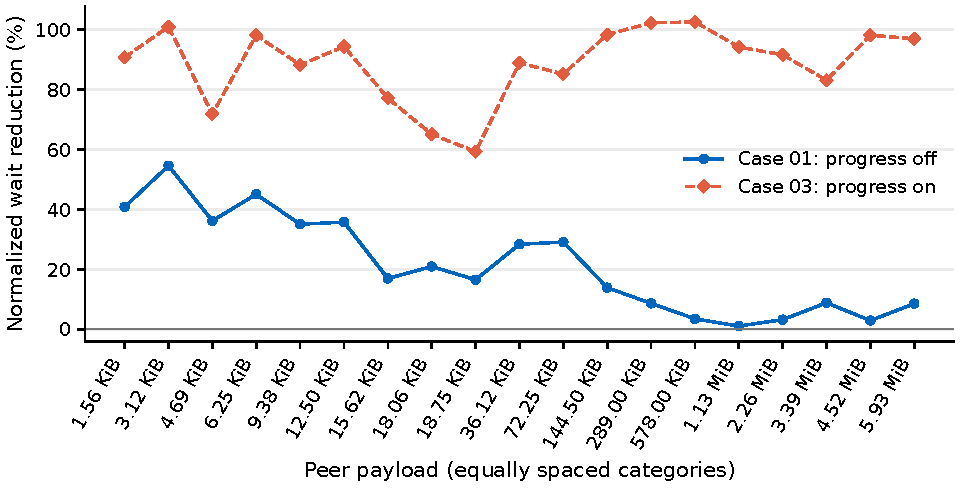
\includegraphics[width=\textwidth]{figures/on_off/inter-intelmpi_tcp-case01-06-overlap-vs-message-size.pdf}
    \caption[Intel MPI TCP asynchronous progress off versus on.]{Intel MPI TCP: measured overlap across 19 peer payloads with
        asynchronous progress disabled (Case~01, solid line with circles,
        24 application threads) and enabled (Case~03, dashed line with diamonds,
        23 application threads and one CPU reserved for progress).
        Both cases use \texttt{wait\_all} and \texttt{seq/seq-seq} in the
        two-node, two-rank \texttt{cm4\_inter} configuration.}
    \label{fig:intelmpi-tcp-progress-on-off}
\end{figure}

\begin{figure}[htbp]
    \centering
    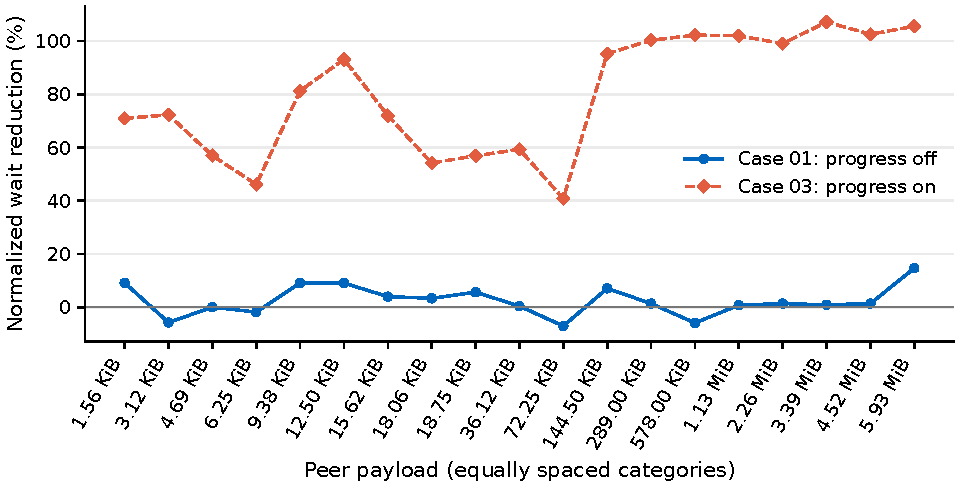
\includegraphics[width=\textwidth]{figures/on_off/inter-intelmpi-case01-06-overlap-vs-message-size.pdf}
    \caption[Intel MPI verbs asynchronous progress off versus on.]{Intel MPI verbs: measured overlap across 19 peer payloads with
        asynchronous progress disabled (Case~01, solid line with circles,
        24 application threads) and enabled (Case~03, dashed line with diamonds,
        23 application threads and one CPU reserved for progress).
        Both cases use \texttt{wait\_all} and \texttt{seq/seq-seq} in the
        two-node, two-rank \texttt{cm4\_inter} configuration.}
    \label{fig:intelmpi-verbs-progress-on-off}
\end{figure}

As shown in Figures~\ref{fig:intelmpi-tcp-progress-on-off} and
\ref{fig:intelmpi-verbs-progress-on-off}, the two Intel MPI transport
configurations exhibit substantially different behavior when asynchronous
progress is disabled.

For Intel MPI TCP, Case~01 shows moderate but irregular overlap in the
small-payload region. At 1.56~KiB, the mean overlap is approximately
41\%, and the values fluctuate between approximately 17\% and 55\% over
much of the remaining small-payload range. As the payload increases, the
overlap generally decreases. From approximately 578~KiB onward, it remains
close to zero for most payloads.

Intel MPI verbs shows a markedly different Case~01 behavior. Across almost
the complete payload sweep, the mean overlap remains close to zero, with
most values lying approximately between -10\% and 15\%. Thus, without
asynchronous progress, the verbs transport provides little sustained
communication--computation overlap during the injected computation window.

Enabling asynchronous progress substantially changes the behavior of both
transport paths. For TCP, Case~03 achieves considerably higher overlap
across almost the entire payload range, with most values lying between
approximately 60\% and 100\%. Unlike Case~01, no systematic collapse toward
zero is observed for large payloads.

The effect is even more pronounced for verbs. Whereas Case~01 remains close
to zero across most payloads, Case~03 exhibits substantial overlap throughout
the sweep. For medium and large payloads, the measured overlap reaches
approximately 95\% to 105\% for most points.

These results indicate that asynchronous progress has a substantial positive
effect on Intel MPI communication--computation overlap for both TCP and verbs.
The effect is particularly strong for the verbs transport, where enabling
asynchronous progress changes $R_{\mathrm{wait}}$ from close to zero to
approximately $100\%$ for many medium and large payloads. At these points,
the receive-wait reduction is approximately equal to the measured computation
time; this does not by itself establish that all communication is hidden.


\subsection{Impact of Completion Strategy: \texttt{wait\_all} versus \texttt{test\_all}}
\label{sec:completion-methods}

In Comb, \texttt{wait\_all} calls \texttt{MPI\_Waitall} to wait for all
communication requests to complete, whereas \texttt{test\_all} repeatedly
calls \texttt{MPI\_Testall} until all requests have completed. Both execute
after the injected computation, so this comparison concerns the communication
completion method rather than polling during computation.

This experiment examines whether replacing \texttt{wait\_all} with
\texttt{test\_all} improves the measured communication--computation overlap
when the injected computation time is approximately equal to the reference
communication time. Case~01 is compared with Case~02 with asynchronous
progress disabled, and Case~03 with Case~04 with progress enabled.

\begin{figure}[htbp]
    \centering
    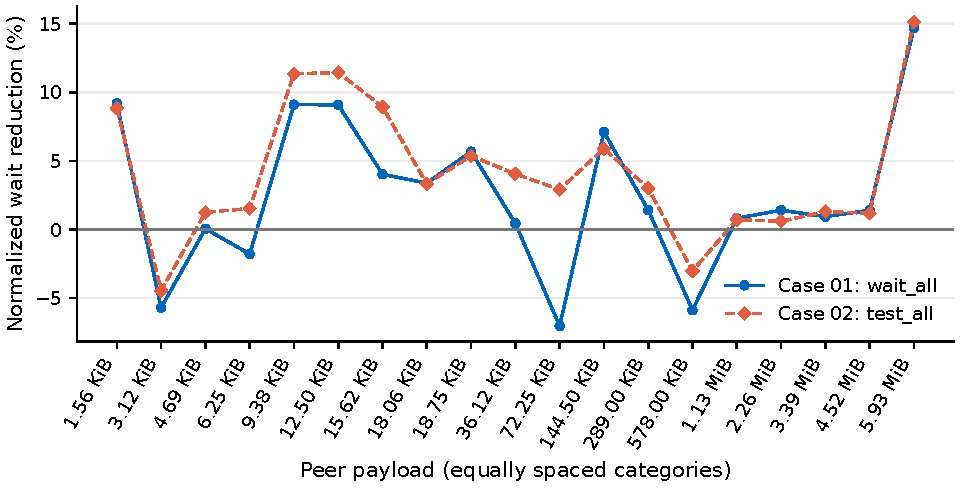
\includegraphics[width=\textwidth]{figures/testall/intelmpi-case01-03-overlap-vs-message-size.pdf}
    \caption[Intel verbs completion comparison with progress disabled.]{Intel
    MPI verbs, Case~01 versus Case~02, with progress disabled and the
    \texttt{seq/seq-seq} policy. Solid blue circles denote \texttt{wait\_all};
    dashed orange diamonds denote \texttt{test\_all}. Points are run
    means.}
    \label{fig:intel-verbs-wait-test-off}
\end{figure}

\begin{figure}[htbp]
    \centering
    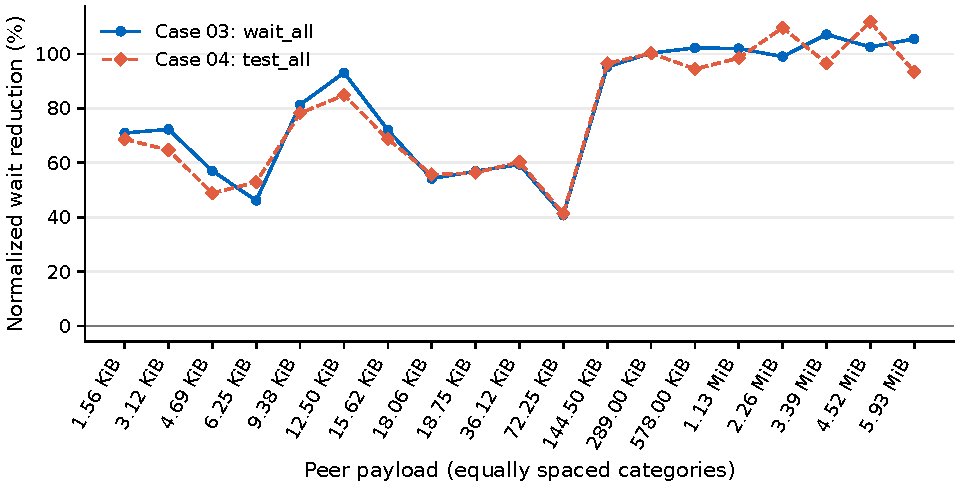
\includegraphics[width=\textwidth]{figures/testall/intelmpi-case06-09-overlap-vs-message-size.pdf}
    \caption[Intel verbs completion comparison with progress enabled.]{Intel
    MPI verbs, Case~03 versus Case~04, with progress enabled and the
    \texttt{seq/seq-seq} policy. Solid blue circles denote \texttt{wait\_all};
    dashed orange diamonds denote \texttt{test\_all}. Points are run
    means.}
    \label{fig:intel-verbs-wait-test-on}
\end{figure}

Under these test conditions, the two completion methods generally show
similar measured overlap. Although differences occur at individual message
sizes, \texttt{test\_all} does not provide a consistent improvement.
The Intel MPI verbs results are shown in
\autoref{fig:intel-verbs-wait-test-off} and
\autoref{fig:intel-verbs-wait-test-on}; the Intel MPI TCP, Open MPI,
and MPICH comparisons are provided in \autoref{app:completion-comparisons}.




\section{Polling During Computation}
\label{sec:compute-polling}
Unlike the computation window described in Section 3.1.3, which contains no explicit MPI progress or completion calls, the polling configuration introduces two polling points at approximately equal intervals within the injected computation. At each point, outstanding receive and send requests are tested using \texttt{MPI\_Testall}, after which computation continues without waiting for all requests to complete. Both cases retain \texttt{wait\_all} for final communication completion.

\subsection{Intel MPI verbs}

Figures~\ref{fig:polling-case01} and \ref{fig:polling-case06} compare
measured overlap with and without polling at four peer payloads for
Case~01 and Case~03, respectively. In the polling configuration, two
\texttt{MPI\_Testall} calls are inserted at approximately equal intervals
within the injected computation. At each polling point, Comb tests the
outstanding receive and send requests and then continues the computation
without waiting for all requests to complete. Both cases use
\texttt{wait\_all} for final communication completion.

\begin{figure}[htbp]

    \centering

    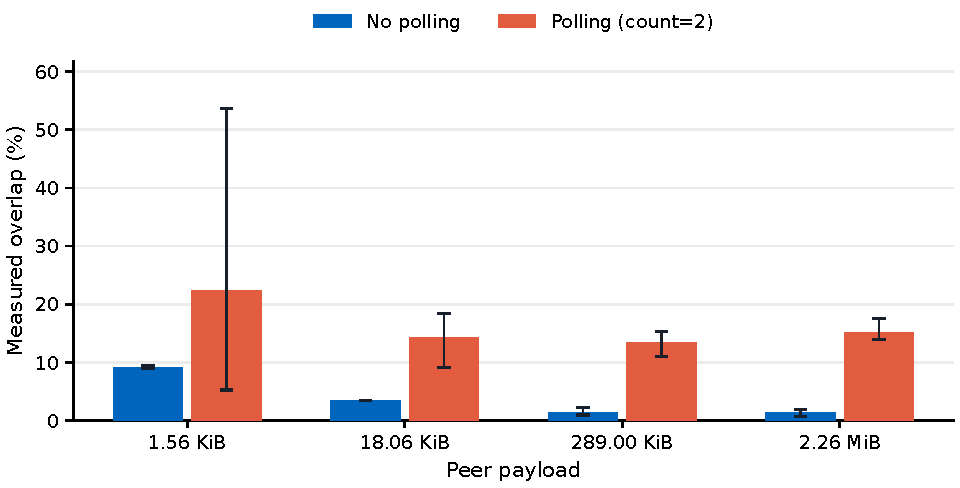
\includegraphics[width=\textwidth]{figures/polling/polling-intelmpi-case01-overlap.pdf}

    \caption[Intel MPI verbs polling with asynchronous progress disabled.]{Intel MPI verbs,
    Case~01: measured overlap with and without two polling points during
    computation. Asynchronous progress is disabled. Bars show run
    means, and error bars show the minimum--maximum range.}

    \label{fig:polling-case01}

\end{figure}

With the asynchronous progress thread disabled in Case~01, the selected
polling results show higher mean overlap at all four payloads. This is
consistent with explicit MPI calls during computation providing additional
opportunities for communication progress in this configuration.

\begin{figure}[htbp]

    \centering

    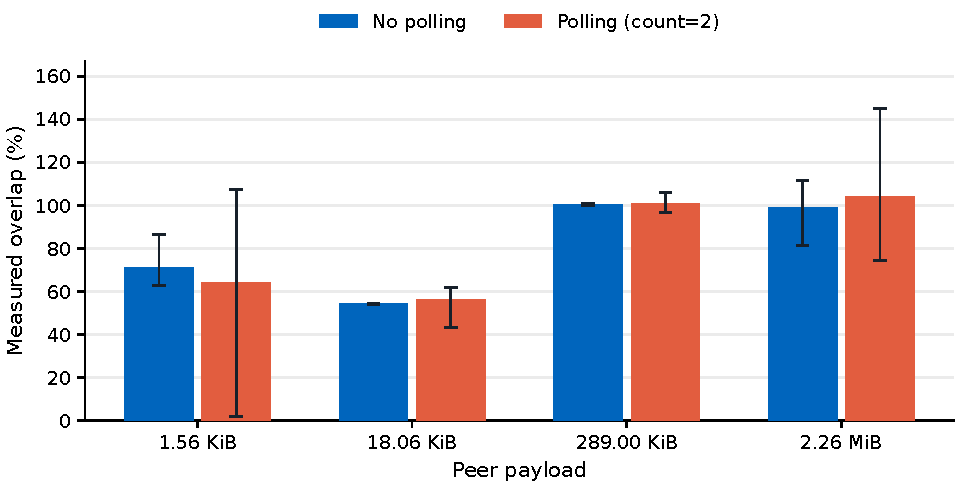
\includegraphics[width=\textwidth]{figures/polling/polling-intelmpi-case06-overlap.pdf}

    \caption[Intel MPI verbs polling with asynchronous progress enabled.]{Intel MPI verbs,
    Case~03: measured overlap with and without two polling points during
    computation. Asynchronous progress is enabled. Bars show run
    means, and error bars show the minimum--maximum range.}

    \label{fig:polling-case06}

\end{figure}


\subsection{Open MPI TCP}

Figures~\ref{fig:polling-openmpi-case01} and
\ref{fig:polling-openmpi-case03} show the results with asynchronous progress
disabled and enabled, respectively.

For Open MPI TCP, inserting two polling points during computation does not provide a consistent improvement in measured overlap. At the two smaller payloads, the mean values with polling remain similar to the corresponding no-polling results. Although polling substantially increases the mean \(R_{\mathrm{wait}}\) at 289.00~KiB when asynchronous progress is disabled, this behavior is not reproduced consistently at the other payloads or when asynchronous progress is enabled.

More importantly, the polling configurations exhibit substantially greater run-to-run variability at several payload sizes. In particular, at 18.06~KiB, 289.00~KiB, and 2.26~MiB, the minimum--maximum ranges are clearly wider than those of the corresponding no-polling measurements. This variability is especially pronounced at 2.26~MiB, where the polling results span both large positive and negative values.

Overall, under the configurations evaluated in this study, the results provide no evidence that explicit polling yields a stable and reproducible overlap benefit for Open MPI TCP. Instead, polling is associated with increased run-to-run variability in \(R_{\mathrm{wait}}\).

\begin{figure}[htbp]
    \centering
    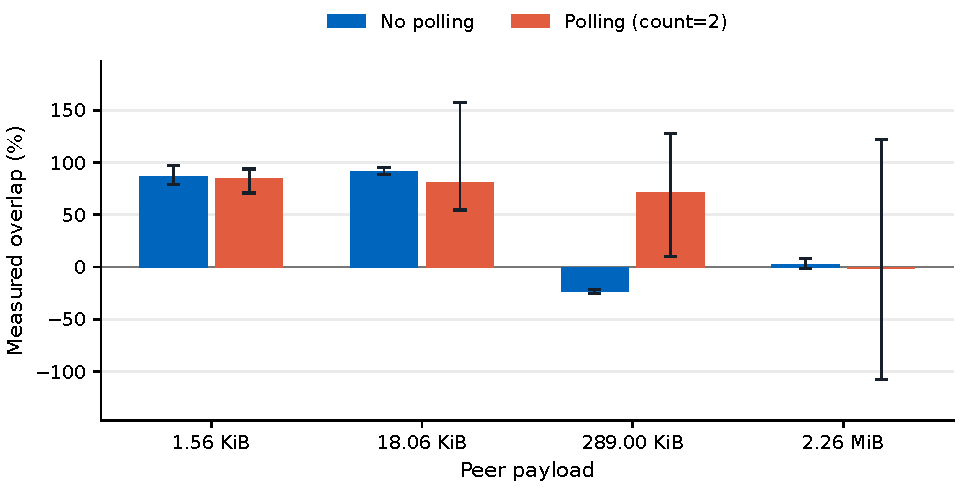
\includegraphics[width=\textwidth]{figures/polling/polling-openmpi-case01-overlap.pdf}
    \caption[Open MPI polling with asynchronous progress disabled.]{Open MPI
    TCP, Case~01: measured overlap with and without two polling points during
    computation. Asynchronous progress is disabled. Bars show means across
    runs, and error bars show the minimum--maximum range.}
    \label{fig:polling-openmpi-case01}
\end{figure}

\begin{figure}[htbp]
    \centering
    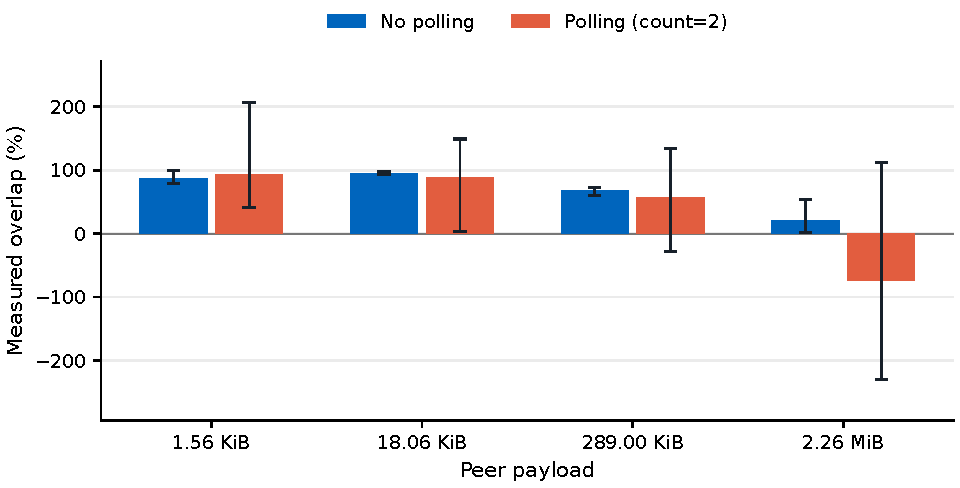
\includegraphics[width=\textwidth]{figures/polling/polling-openmpi-case03-overlap.pdf}
    \caption[Open MPI polling with asynchronous progress enabled.]{Open MPI
    TCP, Case~03: measured overlap with and without two polling points during
    computation. Asynchronous progress is enabled. Bars show means across
    runs, and error bars show the minimum--maximum range.}
    \label{fig:polling-openmpi-case03}
\end{figure}

%\section{Compute-Window Sensitivity}
